\begin{figure*}[tb]
	\centering
	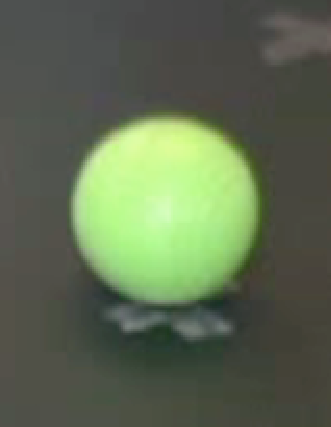
\includegraphics[height=1.75cm]{images/objects/palla}
	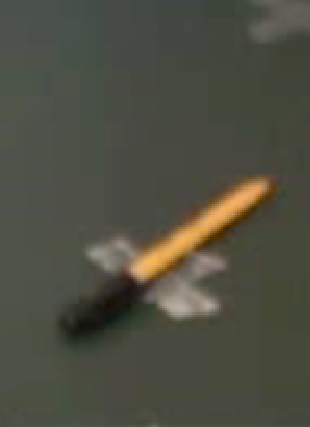
\includegraphics[height=1.75cm]{images/objects/penna}
	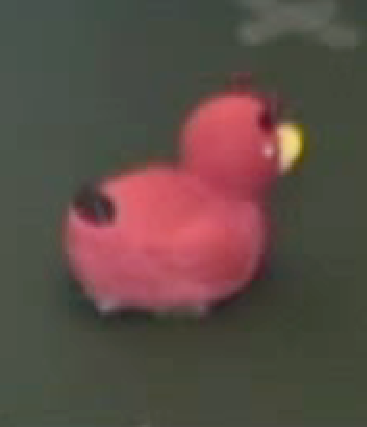
\includegraphics[height=1.75cm]{images/objects/papera}
	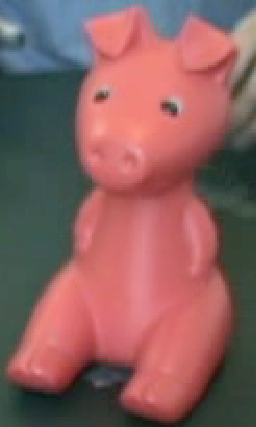
\includegraphics[height=1.75cm]{images/objects/porcellino}
	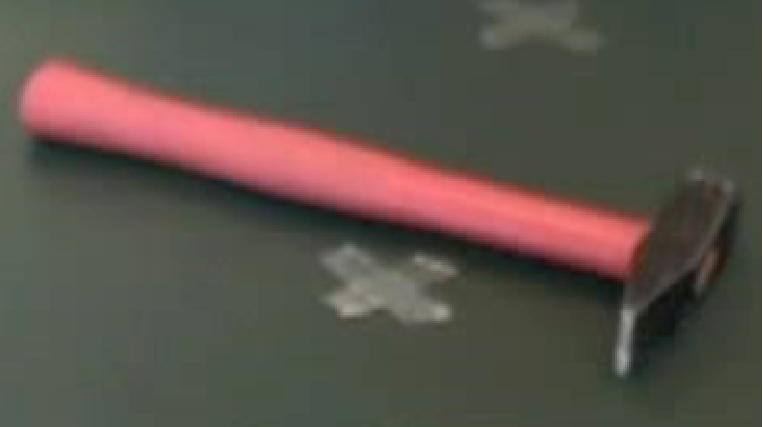
\includegraphics[height=1.75cm]{images/objects/martello}
	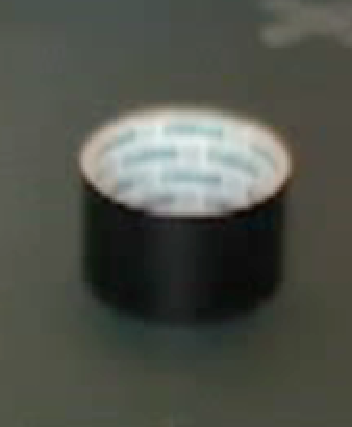
\includegraphics[height=1.75cm]{images/objects/scotch}
	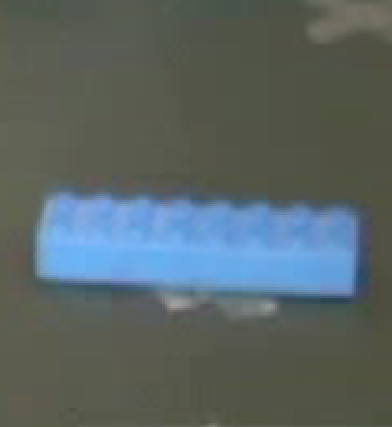
\includegraphics[height=1.75cm]{images/objects/lego}\\
	\vskip 0.1cm
	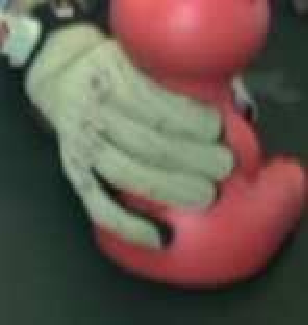
\includegraphics[width=0.12\textwidth]{images/objects/cylinder}
	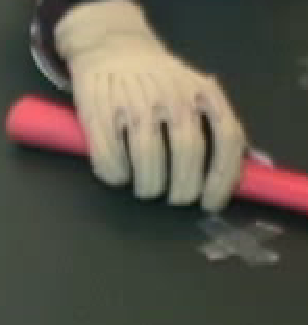
\includegraphics[width=0.12\textwidth]{images/objects/flat}
	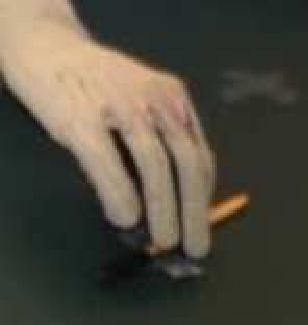
\includegraphics[width=0.12\textwidth]{images/objects/pinch}
	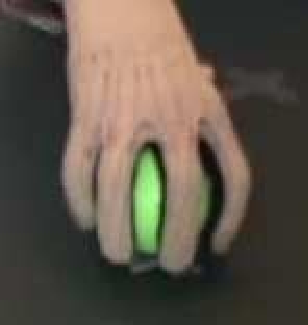
\includegraphics[width=0.12\textwidth]{images/objects/spherical}
	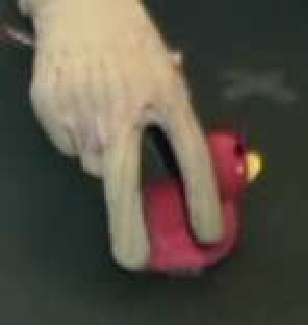
\includegraphics[width=0.12\textwidth]{images/objects/tripodal}
	\caption{Top row: the objects used in our experiments. Bottom, the grasp types we consider: \emph{(left to right)} cylindric power grasp, flat grasp, pinch grip, spherical and
	tripodal grip.}
	\label{fig::grasps}
\end{figure*}

The VMGdB dataset is built considering 7 different objects ((see Fig. \ref{fig::grasps}), top) and 5 grasps ((see Fig. \ref{fig::grasps}), bottom).
 20 different actors participated to the acquisition, during which  
 each object was grasped in one or more  ways, according to the many-to-many relationship reported in Table \ref{tab:manytomany}. In total
we consider 13 different pairs (grasp,object), and, for each triple {\em (object, grasp, actor)}, we acquired 20 replicates of the grasping experiment.
 
 {\small
\begin{table}
\begin{tabular}{c | c c c c c c c}
& ball & pen & duck & pig & hammer & tape & lego brick \\
\hline \\
cylindr. pow. & & & & X & & & \\
flat & & & &  & X & & X \\
pinch & & X & X & & & X & X \\
spherical & X & & & & & X & \\
tripodal & X & X & X & & & X & 
\end{tabular}
\caption{\label{tab:manytomany} Mapping grasps-objects. Each actor performs grasping actions on 13
object-grasp type pairs.}
\end{table}
}
 
We obtained 5200 experiments {\em (object, grasp, actor, expnum)}, and for each of them the VMGdB stores the following information:
\begin{itemize}
\item {\bf Visual information.} 2 video sequences  acquired by 2 color cameras with different focus -- one is the object, the other one is the grasping action. The video sequences
are associated to 2 data files reporting the video frames time-stamps, allowing for synchronization with the sensor data;
\item {\bf Hand posture sensor information.} 1 data file containing the hand posture sensor data acquired by a CyberGlove
\cite{cyberglove}. 
For each posture the glove returns $22$ $8$-bit numbers linearly related to the angles of the actor's hand joints. 
The sensors describe the position of the three phalanxes of each finger (for the thumb, rotation and two phalanxes), the four finger-to-finger
abductions, the palm arch, the wrist pitch and the wrist yaw. Again, the sensor data are associated to acquisition time-stamps for synchronization. 
\end{itemize}

